% -*- TeX-master: "oving04"; -*-
\oppgaver{6}

\begin{oppgave}
Regn ut determinanten til følgende matriser og avgjør -- basert på dette -- om kolonnene er lineært uavhengige:
\begin{punkt}
$$\begin{bmatrix}
1 & 2\\
1 & 2
\end{bmatrix}$$
\end{punkt}

\begin{punkt}
$$\begin{bmatrix}
1 & 2\\
2 & 1
\end{bmatrix}$$
\end{punkt}

\begin{punkt}
$$\begin{bmatrix}
1 & 2 & 3\\
2 & 3 & 4\\
3 & 4 & 5
\end{bmatrix}$$
\end{punkt}

\begin{punkt}
$$\begin{bmatrix}
8 & -7 & 0\\
-8 & -7 & 3\\
-4 & 5 & -8
\end{bmatrix}$$
\end{punkt}

\end{oppgave}

\begin{losning}

\begin{punkt}
0
\end{punkt}

\begin{punkt}
-3
\end{punkt}

\begin{punkt}
0
\end{punkt}

\begin{punkt}
860
\end{punkt}

\end{losning}


\begin{oppgave}
Hva er sammenhengen mellom areal/volum og determinanten? Regn ut og skisser arealet av parallellepipedet utspent av følgende vektorer i $\mathbb{R}^2$:

\begin{punkt}
$$
\begin{bmatrix}
1\\
1
\end{bmatrix} \quad \begin{bmatrix}
2\\
2
\end{bmatrix}$$
\end{punkt}


\begin{punkt}
$$
\begin{bmatrix}
1\\
2
\end{bmatrix} \quad \begin{bmatrix}
2\\
1
\end{bmatrix}$$
\end{punkt}

\end{oppgave}

\begin{losning}

\begin{punkt}
0


\begin{center}
	\begin{tikzpicture}[scale=1]
	\draw[->,above] (0,0) node{} -- (1,1) node{$\vv{1}{1}$};
	\draw[->, right] (0,0) node{} -- (2,2) node{$\vv{2}{2}$};
	%\draw[->, right] (0,0) node{} -- (2,-1) node{$\V{v}_3$};
	\draw[->] (-1,0) {} -- (3,0) {};
	\draw[->] (0,-1) {} -- (0,3) {};
	\end{tikzpicture}
\end{center}
\end{punkt}

\begin{punkt}
3

\begin{center}
	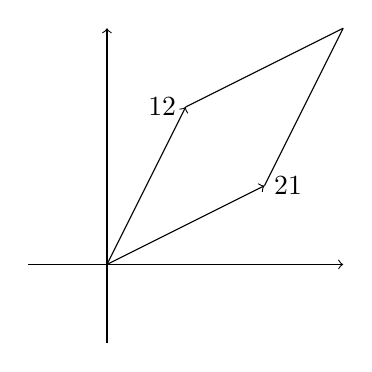
\begin{tikzpicture}[scale=1]
	\draw[->,left] (0,0) node{} -- (1,2) node{$\vv{1}{2}$};
	\draw[->, right] (0,0) node{} -- (2,1) node{$\vv{2}{1}$};
	\draw[] (1,2) node{} -- (3,3);
	\draw[] (2,1) node{} -- (3,3);
	%\draw[->, right] (0,0) node{} -- (2,-1) node{$\V{v}_3$};
	\draw[->] (-1,0) {} -- (3,0) {};
	\draw[->] (0,-1) {} -- (0,3) {};
	\end{tikzpicture}
\end{center}
\end{punkt}


\end{losning}


\begin{oppgave}
La $T$ være tetraederet i $\mathbb{R}^3$ med $(8,8,4)$, $(16,0,0)$, $(1,1,9)$ og~$(8,11,-4)$ som hjørner. Regn ut volumet av $T$.
\end{oppgave}

\begin{losning}
430

\noindent
Hint: Velg et referansepunkt og se på differansen fra de andre vektorene. Du har nå tre vektorer i $\mathbb{R}^3$ som definerer $T$. Observer at $T$ er halvparten av volumet til parallellepipedet definert av vektorene. 
\end{losning}


\begin{oppgave}
La $A$ være matrisen \[
\begin{bmatrix}
\;a & b & 0 & 0\;\\
\;c & 0 & 0 & 0\;\\
\;0 & 0 & 0 & x\;\\
\;0 & 0 & y & z\;
\end{bmatrix}.
\]
\begin{punkt}
Hva er determinanten til $A$ uttrykt ved $a, b, c$ og $x, y, z$?
\end{punkt}

\begin{punkt}
For hvilke verdier av  $a, b, c$ og $x, y, z$ er $A$ inverterbar?
\end{punkt}
\end{oppgave}


\begin{losning}

\begin{punkt}
$bcxy$
\end{punkt}

\begin{punkt}
Vi må ha at $b$, $c$, $x$ og~$y$ alle ikke er lik null.
\end{punkt}

\end{losning}

\begin{oppgave}

Avgjør om følgende påstander er sanne eller ikke. Gi et bevis eller moteksempel i hvert tilfelle.

\begin{punkt}
La $A$ og $B$ være $n\times n$-matriser. Hvis $AB$ er invertibel, så er både $A$ og $B$ invertible.
\end{punkt}

\begin{punkt}
Anta at $A$ er en inverterbar matrise. Da har vi at $$\text{det}(A^{-1})=\frac{1}{\text{det}(A)}.$$
\end{punkt}

\begin{punkt}
Determinanten er definert for alle $m\times n$-matriser.
\end{punkt}

\end{oppgave}

\begin{losning}

\begin{punkt}
Sant.

\noindent
Hint: En matrise er inverterbar hvis og bare hvis determinanten ikke er lik null. Vi vet også at $\text{det}(AB)=\text{det}(A)\text{det}(B)$. Vi har antatt at $\text{det}(AB)\neq 0$. Kan du fullføre beviset?
\end{punkt}

\begin{punkt}
Sant.

\noindent
Hint: $AA^{-1}=I$ og $\text{det}(AB)=\text{det}(A)\text{det}(B)$.
\end{punkt}

\begin{punkt}
Feil; determinanten er kun definert dersom $m=n$.
\end{punkt}

\end{losning}
